\section{Hintergrund}
Der Fußschalter soll in einer komplexen Umgebung aus Messwerkzeug und Computer agieren, weshalb in diesem Kapitel zum Verständnis wichtige Hintergrundinformationen gegeben werden sollen. Es wird \ac{BLE} vorgestellt, dass die Grundtechnologie für den Informationsaustausch zwischen Fußschalter und dem Messwerkzeug darstellt, sowie die \ac{HCT}-Plattform und das \ac{HCT}-Protokoll auf dem sie aufbaut.

\subsection{Bluetooth Low Energy}
Dabei wurde sich für \ac{BLE} enschieden, da den Hand- und Messwerkzeugen, aufgrund ihrer handlichkeit und nicht kabelgebundenheit, nur begrenzte Batteriespeicherkapazitäten zu Verfügung stehen. \ac{BLE} ist eine Abwandlung des klassischen Bluetooth und ist besonders auf Energiesparkeit hin optimiert, wodurch es auch auf dem Hand- und Messwerkzeug lange Batterielaufzeiten garantieren kann.

\subsection{HCT-Plattform}
Um die Digitalisierung der Messergebnisse dem Anwender so einfach wie möglich zu gestalten, setzt die Hoffmann Group mit der \ac{HCT}-Plattform darauf, die Digitalisierung der durchgeführten Arbeitsschritte als einen festen Bestandteil in ihr Werkzeug zu integrieren. Diese sind zum Stand dieser Arbeit: 
\begin{itemize}
	\item Drehmomentschlüssel
	\item Messschieber bzw. Messuhren
	\item Drehmomentprüfgerät
	\item Bügelmessschrauben
\end{itemize}
Sie stellen dem Anwender die Daten der Messungen in verschiedener Weise zu Verfügung. Zum Einen können die Geräte als ein \ac{HID} über \ac{BLE} mit dem Computer verbunden werden. Sie simulieren dann eine über Bluetooth verbundene Tastatur über die, die Messergebnisse als Tastendrücke serialisiert werden. Das Messergebnis kann dann in einem Texteditor oder Excel aufgefangen werden. Des weiteren erzeugen die Drehmomentschlüssel und das Drehmomentprüfgerät eine \ac{CSV}-Datei, in der alle durchgeführten Messungen mit einer großen Anzahl an zusätzlichen Daten gespeichert werden. Wird das Gerät über \ac{USB} mit dem Computer verbunden, zeigt es sich als \ac{MSC}-Device und die Datei kann per Drag-and-drop auf den Computer kopiert werden. Eine weitere Möglichkeit die durchgeführten Messungen zu digitalisieren, ist mithilfe der \ac{HCT}-Windows-App. Diese erfordert zusätzlich zur frei verfügbaren Software einen speziellen Dongle der zum Verbinden der Geräte benötigt wird. Sie werden ebenfalls über \ac{BLE} verbunden und sprechen über \ac{BLE} das firmeneigene \ac{HCT}-Protokoll. Die Windows-App bietet zahlreiche Möglichkeiten die Messdaten zu digitalisieren und den Produktionsprozess zu optimieren. Es können Schraubfälle in der App angelegt werden und mit Bildern hinterlegt werden. Die Seriennummer von Werkstücken kann automatisch mit dem dazugehörigen Messwert verlinkt werden und \ac{CAQ}-Software kann über einen virtuelle COM-Port angebunden werden. Die \ac{HCT}-Windows-App unterstützt derzeit lediglich die Drehmomentschlüssel, jedoch ist die Einbindung der restlichen \ac{HCT}-Geräte in Entwicklung. Der Fußschalter und der Dongle nehmen dabei eine ähnliche Position, jedoch mit geringerem Funktions- und Userinterfaceumfang, wie die Windows-App ein. Der letzte Baustein der \ac{HCT}-Plattform ist die \ac{HCT}-Mobile-App, sie ist ebenfalls frei erhältlich und erleichtert vorallem die Bedienung des Geräts, zum Beispiel bei Arbeitsschritten bei denen das Display des Werkzeugs für den Anwender nicht sichtbar ist.

\subsection{HCT-Protokoll}
Der \ac{HCT}-Plattform liegt das firmeneigene \ac{HCT}-Protokoll zugrunde. Es stellt sicher, dass alle Geräte der \ac{HCT}-Plattform stets kompatibel zu einander sind. Es ist ein binäres Protokoll, dass entwickelt wurde um über \ac{BLE} gesprochen zu werden und stellt ein virtuelles Speichermodel der Geräte da. Dabei besitzten Werkzeuge unterschiedlicher Produktreihen und Hersteller jeweils verschiedene Speichermodelle. Über ``read'' und ``write'' Befehle auf die Speicheradressen kann dann der interne Zustand des Werkzeug abgefragt und verändert werden. So können auch komplexe Operationen effizient über \ac{BLE} durchgeführt werden. Zudem stehen automatisierte Tools zur Verfügung mit deren Hilfe die Frameworks, die das Sprechen des HCT-Protokoll abstrahieren, um die Speichermodelle neu eingeführter Werkzeuge erweitert werden kann.
\begin{figure}[H] 
	\centering
	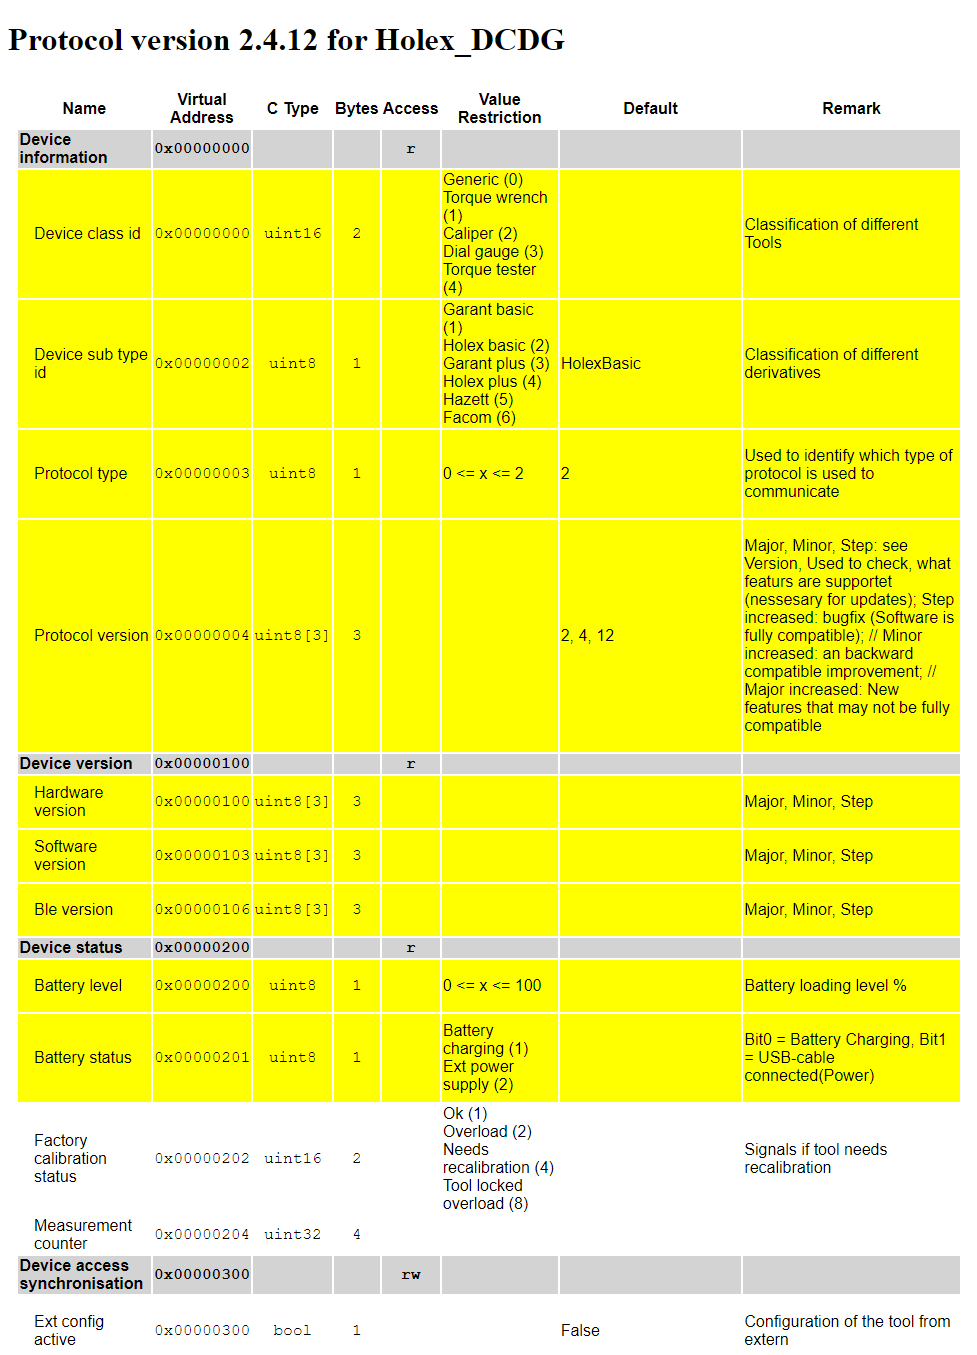
\includegraphics[width=\textwidth]{figures/HCT_Protocol_DCDG.png}
	\caption{Auszug aus dem virtuellen Speichermodell für Messuhren und Messschieber}
\end{figure}